\chapter{Coupled Results}
\label{ch:coupledResults}

\section{Power Reactor Modeling}
\label{sec:power_reactor_modeling}
  The motivation for this work is to model nuclear power reactors with
  multiphysics feedback. This has been accomplished by modeling power
  distribution with the multigroup neutron diffusion equation solved via the
  Finite Element Method (FEM) (\chref{ch:neutronDiffusion}), axial heat
  convection and radial heat conduction models (\chref{ch:thermalHydraulics}),
  and simplified thermal expansion modeling (\chref{ch:thermalExpansion}).
  Combined, these effects will provide feedback which can be estimated in the
  model. 
  
  A realistic reactor benchmark is provided and modeled \sref{sec:abr}.
  Reactivity coefficients describing system responses are defined in
  \sref{sec:reactivity_coefficients}. Results are presented in
  \sref{sec:results}.

\section{Advance Burner Reactor -- MET 1000}
\label{sec:abr}
  This problem is proposed by Organisation for Economic Co-operation and
  Development Nuclear Energy Agency (OECD NEA) in \cite{abr}. The Advanced
  Burner Reactor (ABR) is fueled with a ternary metallic fuel and has a 1000
  \units{MWth} rating. This is a medium-sized metalic reactor with a total of
  180 assemblies and is 4.8 \units{m} tall. The benchmark is fully specified and
  thirty-one independent results are submitted. 
  
  Each submission has generated its own cross-sections using several different
  cross-section libraries (e.g. ENDFB7.0, JEFF3.1, etc.). 
  Cross sections were generated for this model using \mcc and the procedure 
  outlined in \sref{sec:cross_section_treatment}. The reactor multigroup 
  neutron diffusion equation is solved in \dif and using the method from
  \chref{ch:neutronDiffusion} and the methods agree to within 700 \units{pcm}. 
  The solution from the Finite Element Method as implemented in this work is 
  $\keff = 1.006694$.

  The materials in the benchmark are shown in \fref{fig:abr_materials}. Fast
  neutron flux is shown to peak in the core center and thermal neutron flux is
  shown to peak in the structural material surrounding the core in
  \fref{fig:abr_fluxes}.

  \begin{figure}
    \centering
    
\includegraphics[width=0.4\textwidth]{abr_materials}
    \caption{Materials in ABR.}
    \label{fig:abr_materials}
  \end{figure}

  \begin{figure}
    \centering
    \subfloat[$\phi_{1}$]{
      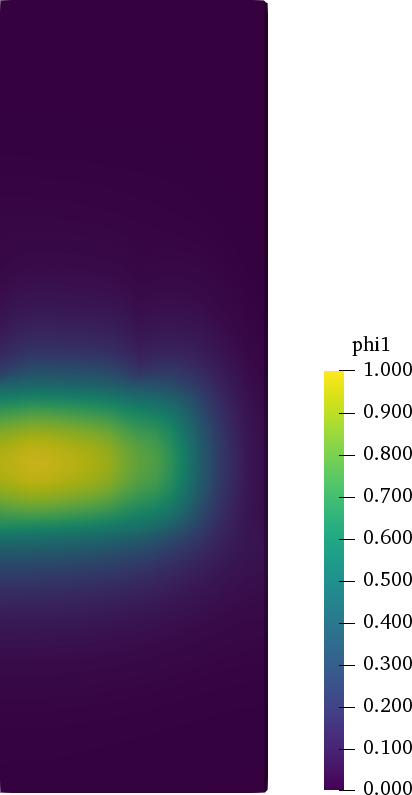
\includegraphics[width=0.25\textwidth]{abr_phi_nod_group1}}
    \hspace{0.2in}
    \subfloat[$\phi_{33}$]{
      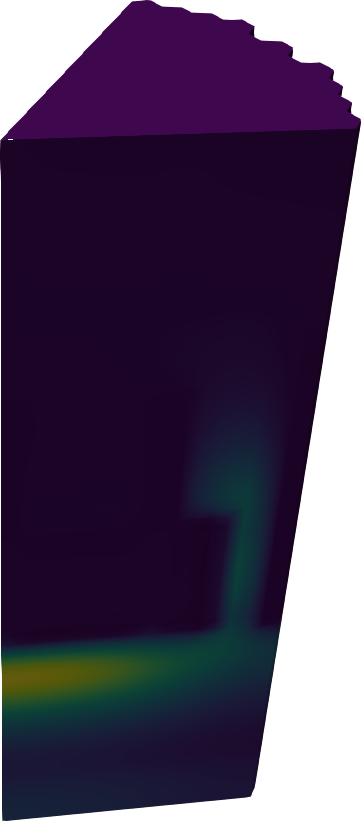
\includegraphics[width=0.25\textwidth]{abr_phi_nod_group33}}
    \caption{Multigroup Neutron Flux in ABR.}
    \label{fig:abr_fluxes}
  \end{figure}

\section{Reactivity Coefficients}
\label{sec:reactivity_coefficients}
  Reactivity of a reactor serves to compare the state of the reactor to the
  critical state.
  \begin{equation}
    \label{eq:reactivity}
    \rho \units{pcm} = \frac{\keff-1}{\keff} \times 10^5
  \end{equation}
  Recall $\keff < 1$ for a subcritical reactor, $\keff=1$ for a critical
  reactor, and $\keff > 1$ for a supercritical reactor. Therefore $\rho < 0$
  for a subcritical reactor, $\rho = 0$ for a critical reactor, and $\rho > 0$
  for a supercritical reactor. 

  A reactivity coefficient can be defined as a partial derivative with respect
  to a quantity of interest \cite{textbookknief}. Let $\alpha_x$ be the 
  reactivity coefficient for quantity $x$, then
  \begin{equation}
    \label{eq:reactivity_coefficient}
    \alpha_x(x_i) = \left. \frac{\partial \rho}{\partial x} \right|_{x_i}
  \end{equation}
  where $\rho$ is the reactivity defined by \eref{eq:reactivity}.
  \eref{eq:reactivity_coefficient} is useful for estimating reactor behaviors.
  For some change in reactor state $\Delta x$, the reactivity response can be
  estimated as 
  \begin{equation}
    \label{eq:reactivity_estimate}
    \Delta \rho \approx \alpha_x(x_i) \, \Delta x.
  \end{equation}
  It is expected that reactivity coefficients will vary as reactor conditions
  vary. Therefore, it will be necessary to calculate $\alpha_x$ as a function of
  reactor condition $x_i$. Specifically, reactor power, $Q_{Rx}$, will be varied 
  in the calculation of $\alpha$. Therefore, consider a set of reactor powers
  varying from $0\%$ to $100\%$ as $Q_{Rx,i} = \{0\%,\ldots,100\%\}$.

  Reactivity coefficients useful for Fast Reactor (FR) applications include the
  power coefficient, thermal expansion coefficient, fuel temperature (Doppler)
  coefficient, and coolant temperature coefficient (CTC) \cite{textbookknief}.
  Reactivity coefficients will be estimated with a first-order, forward-Euler,
  finite-difference approximation such that
  \begin{equation}
    \label{eq:reactivity_coefficient_finite_difference}
    \alpha_x(x_i) \approx \frac{\rho(x_i) - \rho(x_i + \Delta x)}{\Delta x}
  \end{equation}
  for a given $\Delta x$. The parameter $x$ that is varied will depend on the
  coefficient $\alpha_x$ and the evaluation of
  \eref{eq:reactivity_coefficient_finite_difference} is discussed in the
  following sections for relevant reactivity coefficients.

  \subsection{Power Reactivity Coefficient}
  \label{sec:power_reactivity_coefficient}
    The power reactivity coefficient measures the reactivity response due to a 
    power increase. In a stable reactor, $\alpha_{power} < 0$ to ensure an 
    increase in reactor power requires a reactivity increase and to prevent a 
    runaway power increase. Evaluation of $\alpha_{power}$ requires two values 
    of $\keff$ : the first at a nominal reactor power, $\keff(Q_{Rx,i})$, and 
    the second at an increased reactor power 
    ${\keff(Q_{Rx,i} + \Delta Q_{Rx})}$.  These \keff values correspond to 
    reactivities $\keff(Q_{Rx,i})$ and ${\rho(Q_{Rx,i} + \Delta Q_{Rx})}$ 
    respectively as described by \eref{eq:reactivity}. Then, the power 
    reactivity coefficient can be calculate as
    \begin{equation}
      \label{eq:power_reactivity_coefficient}
      \alpha_{power}(Q_{Rx,i}) = \frac{\rho(Q_{Rx,i}) - \rho(Q_{Rx,i} + 
        \Delta Q_{Rx})} {\Delta Q_{Rx}}.
    \end{equation}
    A typical value of $\Delta Q_{Rx}$ is $10\% \, Q_{Rx,i}$.


  \subsection{Thermal Expansion Reactivity Coefficient}
  \label{sec:thermal_expansion_reactivity_coefficent}
    The thermal expansion reactivity coefficient describes the reactivity 
    response due solely to thermal expansion for a given increase in reactor 
    power. It is expected that thermal expansion will be the dominant 
    contribution to the total power reactivity coefficient. This is due to two 
    main reasons: metal fuels expand significantly at high temperature (see 
    \chref{ch:thermalExpansion}) and the large neutron leakage fraction 
    (\leakage) in FRs \cite{PlentifulEnergy}. The leakage fraction is the 
    fraction of neutrons born in the fuel due to fission that exit the core. 
    Light Water Reactors (LWRs) typically have $\leakage \approx 2 \%$ 
    \cite{textbookknief}. However, FRs simulated in this work have 
    $\leakage \approx 20\%$ and therefore are therefore highly sensitive to 
    decreases in fuel density and changing reactor dimensions due to thermal 
    expansion.

    Thermal expansion temperatures, \texpfuel and \texpstruct, as implemented in 
    \chref{ch:thermalExpansion} must be known before the simulation. Therefore,
    the case used to calculate $\keff(Q_{Rx_i} + \Delta Q_{Rx})$ can be used to
    calculate these temperatures. Then, the thermal expansion reactivity
    coefficient is 
    \begin{equation}
      \label{eq:thermal_expansion_reactivity_coefficient}
      \alpha_{thexp}(Q_{Rx,i}) = \frac{\rho(\texp(Q_{Rx,i})) - 
        \rho(\texp(Q_{Rx,i} + \Delta Q_{Rx}))}
        {\Delta Q_{Rx}}
    \end{equation}
    where $\texp(Q_{Rx,i})$ represents the thermal expansion temperatures for
    power $Q_{Rx,i}$ and $\texp(Q_{Rx,i} + \Delta Q_{Rx})$ represents the
    thermal expansion temperatures for power $Q_{Rx,i} + \Delta Q_{Rx}$. Note
    that in \eref{eq:thermal_expansion_reactivity_coefficient}, only thermal
    expansion temperatures are changed, not the true reactor power $Q_{Rx}$.
    A typical value of $\Delta Q_{Rx}$ is $10\% \, Q_{Rx,i}$.

  \subsection{Fuel Temperature (Doppler) Reactivity Coefficient}
  \label{sec:fuel_temperature_reactivity_coefficient}
    The fuel temperature reactivity coefficient measures the reactivity change due
    to an increase in fuel temperature. This coefficient is often termed the
    Doppler coefficient because the reactivity effect is due to the Doppler
    broadening of resonance absorption peaks in heavy nuclei such as
    \isotope[238]{U} \cite{textbookknief}. Briefly, at high fuel temperatures, 
    neutrons are more likely to be parasitically absorbed by non-fissile nuclei
    than fissile-nuclei in the fuel material.

    To calculate $\alpha_{Doppler}$, fuel temperature is increased directly. A
    simulation is conducted with feedback for reactor power $Q_{Rx,i}$ and the
    temperature profile is stored. Then, the fuel temperature is uniformly 
    increased in the reactor by $\Delta T_{fuel}$ and the simulation is
    conducted again. This procedure will result in $\keff(Q_{Rx,i})$ and
    ${\keff(T_{fuel} + \Delta T_{fuel})}$. Associated reactivities can be
    calculated from \eref{eq:reactivity} and the Doppler reactivity coefficient
    follows.
    \begin{equation}
      \label{eq:doppler_reactivity_coefficient}
      \alpha_{Doppler}(Q_{Rx,i}) = \frac{\rho(Q_{Rx,i}) - \rho_i(T_{fuel} +
        \Delta T_{fuel})} {\Delta T_{fuel}}
    \end{equation}
    A typical value of $\Delta T_{fuel}$ is $20\units{K}$.

  \subsection{Coolant Temperature Reactivity Coefficient (CTC)}
  \label{sec:coolant_temperature_reactivity_coefficient}
    Hello.
    \begin{equation}
      \label{eq:coolant_temperature_reactivity_coefficient}
      \alpha_{CTC}(Q_{Rx,i}) = \frac{\rho(Q_{Rx,i}) - \rho(T_{cool} + 
        \Delta T_{cool})} {\Delta T_{cool}}
    \end{equation}

\section{Results}
\label{sec:results}
  The figure is \fref{fig:abr_reactivity_coefficients}. The power reactivity
  coefficient is \fref{fig:power_reactivity_coefficient}.

  \begin{figure}
    \centering
    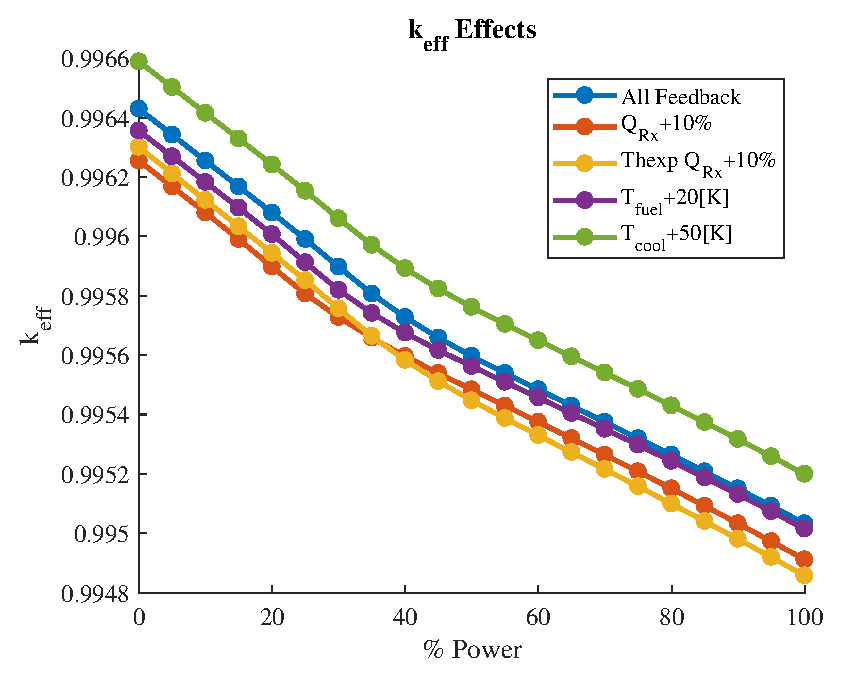
\includegraphics[width=0.7\textwidth]{keff_effects}
    \caption{Feedback Effects on \keff.}
    \label{fig:keff_effects}
  \end{figure}

  \begin{figure}
    \centering
    \subfloat[Power Reactivity Coefficient.]{
      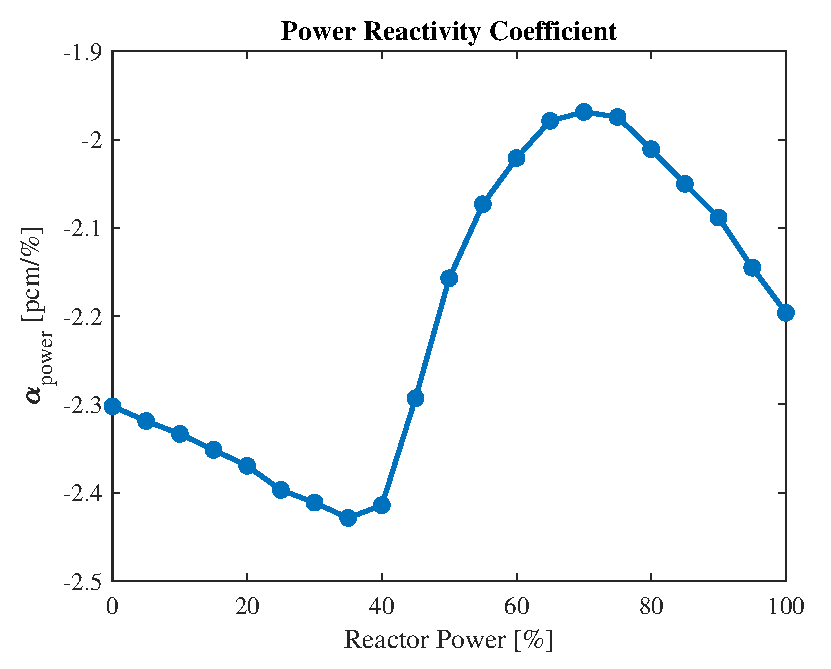
\includegraphics[width=0.5\textwidth]{alpha_power}
      \label{fig:power_reactivity_coefficient}}
    \hspace*{\fill}
    \subfloat[Thermal Expansion Reactivity Coefficient.]{
      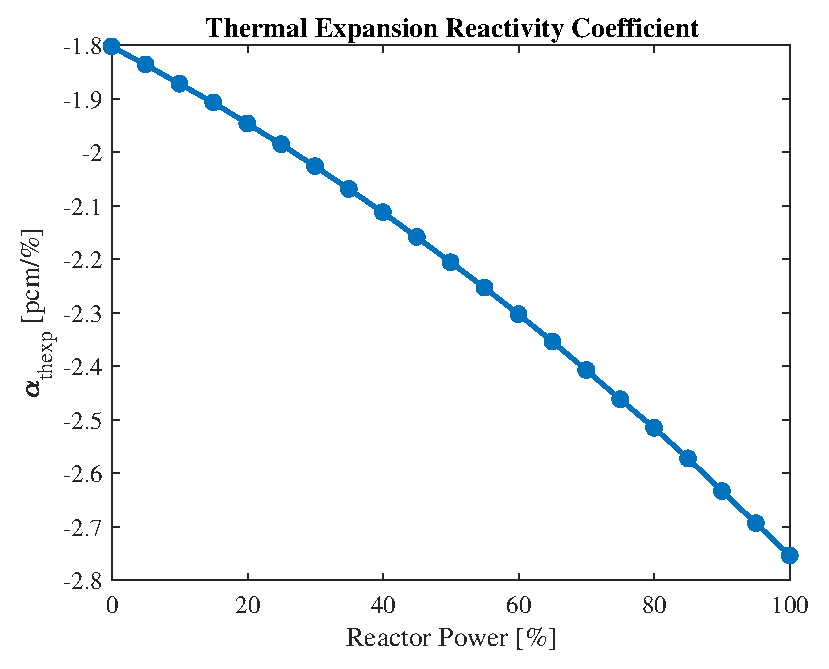
\includegraphics[width=0.5\textwidth]{alpha_thexp}
      \label{fig:thermal_expansion_reactivity_coefficient}}
    \vspace{\baselineskip}
    \subfloat[Doppler Reactivity Coefficient.]{
      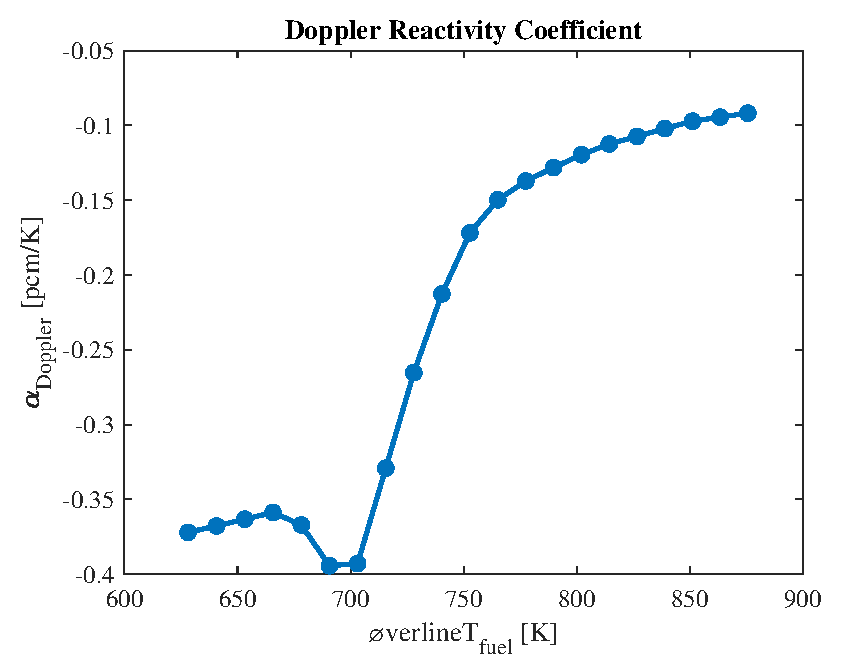
\includegraphics[width=0.5\textwidth]{alpha_fuel}
      \label{fig:doppler_reactivity_coefficient}}
    \hspace*{\fill}
    \subfloat[Coolant Temperature Reactivity Coefficient.]{
      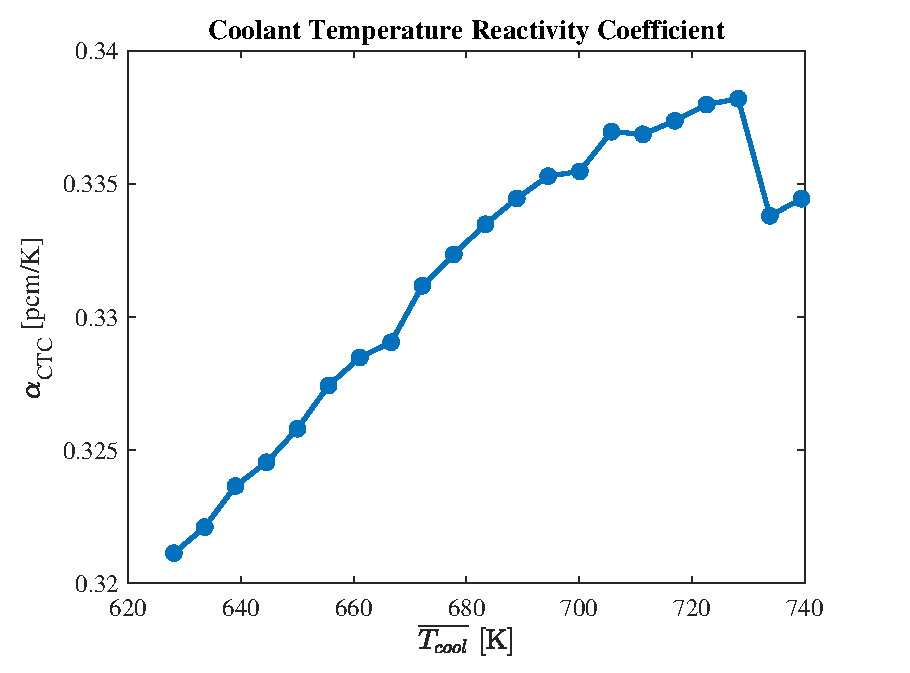
\includegraphics[width=0.5\textwidth]{alpha_cool}
      \label{fig:coolant_temperature_reactivity_coefficient}}
    \caption{ABR Reactivity Coefficients.}
    \label{fig:abr_reactivity_coefficients}
  \end{figure}
